Pro porovnání implementací byla provedena měření výpočetního času.
Všechna měření byla provedena na clusteru \textbf{STAR}.
Byl nám poskytnuty skripty pro spouštění našich aplikací.
Jeden uzel byl přiřazen sekvenčním a paralelním implementacím a distribuovaná implementace mohla používat až 4 uzly.
Každý uzel se skládá z 20 jader.

Doba výpočtu musela být měřena aplikací a k tomu byla použita funkce \texttt{measure\_duration} (viz \ref{lst:measure_duration}.
Přebírá funkci \texttt{find}, která jako výsledek vrací nejlepší stav.
Vrací strukturu \texttt{result}, který se skládá z nejlepšího stavu a doby výpočtu v sekundách.
Čas je měřen pomocí instancí \texttt{std::chrono::high\_resolution\_clock} ze standardní knihovny.

\begin{lstlisting}[language=C++, label={lst:measure_duration}, title={Funkce pro měření doby výpočtu}]
    result measure_duration(const std::function<finder::state()>& find)
    {
        auto begin = std::chrono::high_resolution_clock::now();
    
        auto best = find();
    
        auto end = std::chrono::high_resolution_clock::now();
        auto duration = std::chrono::duration_cast<std::chrono::nanoseconds>(end-begin);
    
        return result(best, duration.count()*1e-9);
    }
\end{lstlisting}

Výsledky každého spuštění aplikace byly uloženy jako řádek instance třídy \texttt{table}, která byla následovně uložena pomocí funkce třídy \texttt{csv} do souboru.
Formát CSV byl použit z důvodu snadného použití ve vizualizační části vyhodnocení výsledků.
Funkce \texttt{run\_sequantial} (viz \ref{lst:run_sequential}) ukazuje, jak se výsledky ukládají.

\begin{lstlisting}[language=C++, label={lst:run_sequential}, title={Funkce pro měření doby výpočtu}]
    void run_sequential(...)
    {
        ....
    
        // prepare table
        pdp::table<std::string, int, int, double> table{
                {"filename", "n vertices", "n edges", "time[s]"}
        };
    
        ....
    
        // save results to csv
        table.add_row({graph_path.filename(), graph.n_vertices(), graph.n_edges(), res.duration});
        pdp::csv csv{csv_path};
        csv.write(table);
    }
\end{lstlisting}

Pro porovnání implementací bylo nutné vybrat alespoň 3 grafy, které běžely 1 až 10 minut na clusteru pomocí sekvenční implementace.
Jelikož všechny testovací grafy, které nám byly poskytnuty, běžely rychleji nebo pomaleji, bylo nutné vygenerovat grafy nové.
Bylo vygenerováno přes sto grafů a 4 z nich, které běžely nejpomaleji, byly vybrány pro porovnání implementací.
Paralelní implementace byly spuštěny pro 1, 2, 4, 6, 8, 12, 16, 20 vláken.
Distribuovaná implementace byla spuštěna na 4 procesech a slave procesy měly přístup k 6, 8, 12, 16, 20 vláknům.
Pro všechna nastavení byl spuštěn každý graf.
Výsledky uložené v souborech csv byly poté vizualizovány pomocí jazyka \texttt{Python} a knihoven, jako jsou \texttt{Pandas}, \texttt{Matplotlib} a \texttt{Seaborn}.

Pro srovnání doby výpočtu byl zvolen sloupcový graf.
Porovnání doby výpočtu pro sekvenční řešení je vidět na grafu \ref{fig:seq-graph.png}.
Pořadí grafů zůstává pro snazší čitelnost stejné pro grafy, které následují.
Lze pozorovat, že nalezení nejlepšího stavu u prvního grafu trvá o poznání déle než u ostatních grafů, jejichž doba výpočtu je přibližně stejná.

\begin{figure}[!htbp]
\centerline{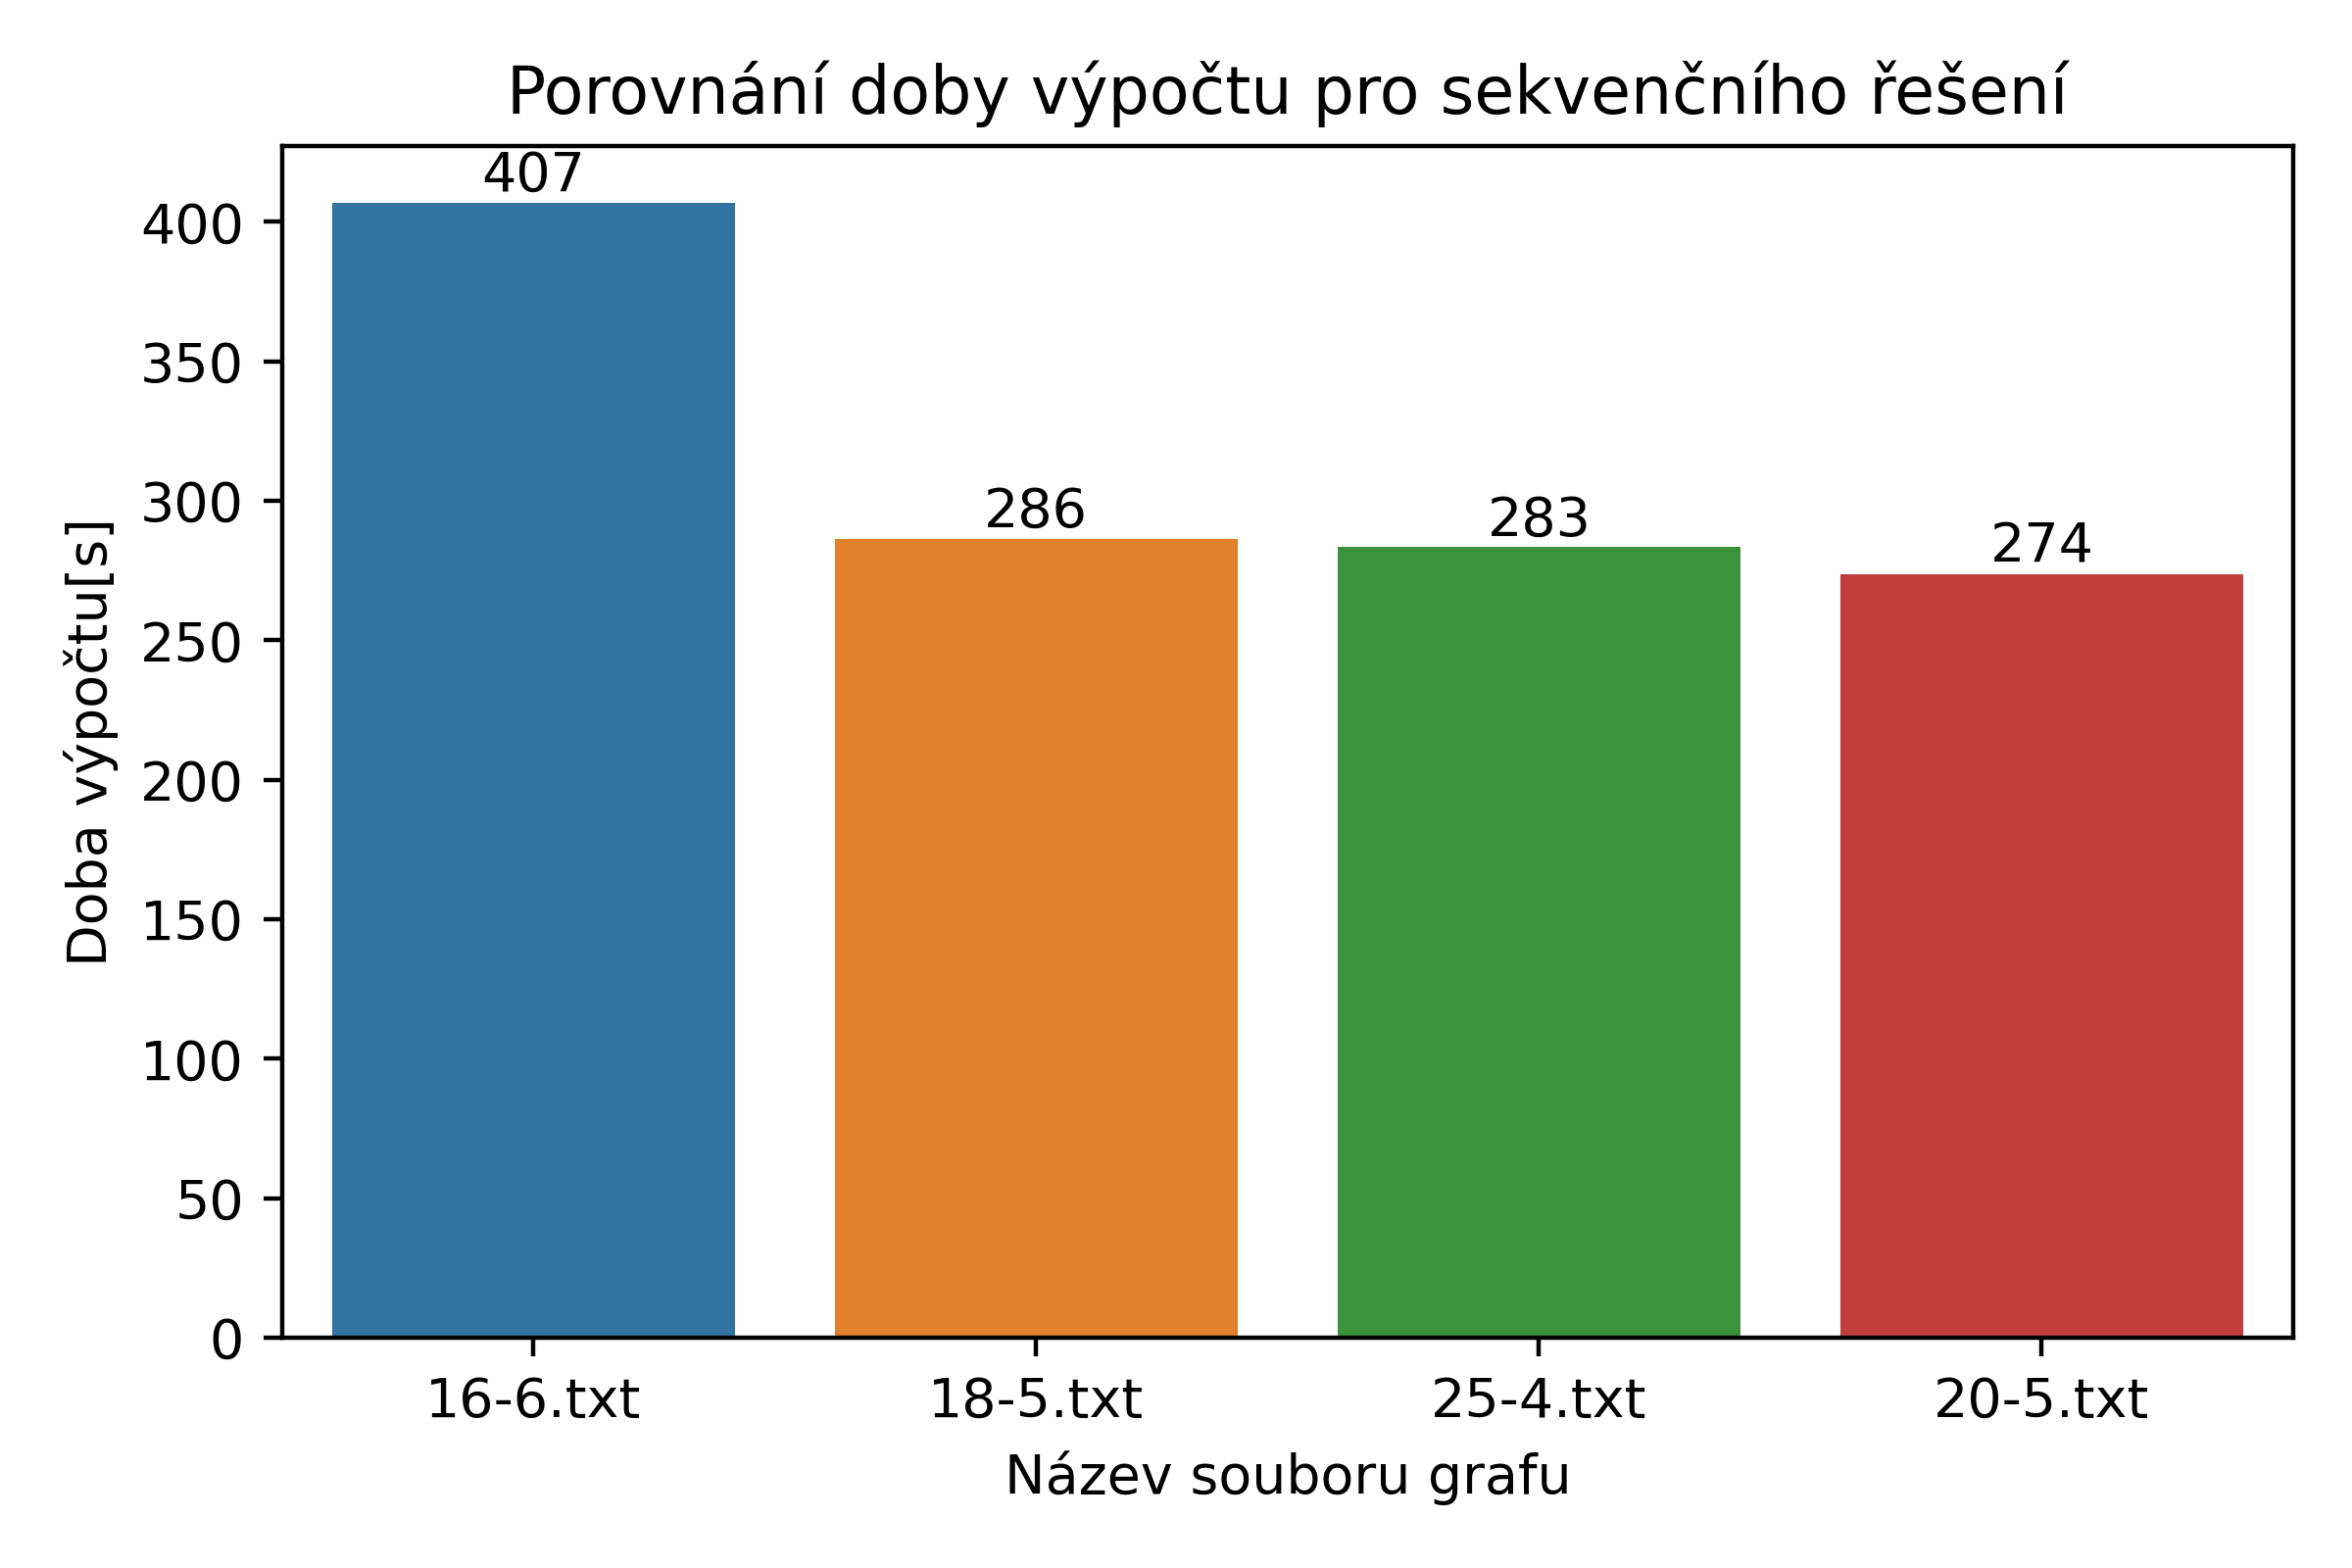
\includegraphics[scale=0.56]{report/images/seq-graph.png}}
\caption{Porovnání doby výpočtu pro sekvenční řešení}
\label{fig:seq-graph.png}
\end{figure}
\FloatBarrier

Následovalo srovnání implementace taskového paralelismu.
Poměr sekvenčně hledaných stavů byl nastaven na \textbf{0,5} na základě experimentů provedených v průběhu semestru.
Z grafu (viz \ref{fig:task-graph.png}) je na první pohled vidět, že se zvyšujícím se počtem vláken se zkracovala doba výpočtu.
V prvním grafu lze pozorovat, že chybí sloupec pro dvě vlákna, což je způsobeno překročením časového limitu.
Z nějakého důvodu byl běh se dvěma vlákny mnohem pomalejší než s jedním vláknem, a to platilo pro všechny grafy.
Po použití alespoň 4 vláken byla paralelní implementace rychlejší než sekvenční.
Při použití několika málo vláken je tedy režie tak vysoká, že se nevyplatí spouštět algoritmus paralelně.
V průměru pro všechny grafy byl nejrychlejší běh zhruba \textbf{dvakrát} rychlejší než sekvenční, což lze považovat za dobrý výsledek vzhledem k tomu, že v kódu bylo provedeno pouze několik málo změn.

\begin{figure}[!htbp]
\centerline{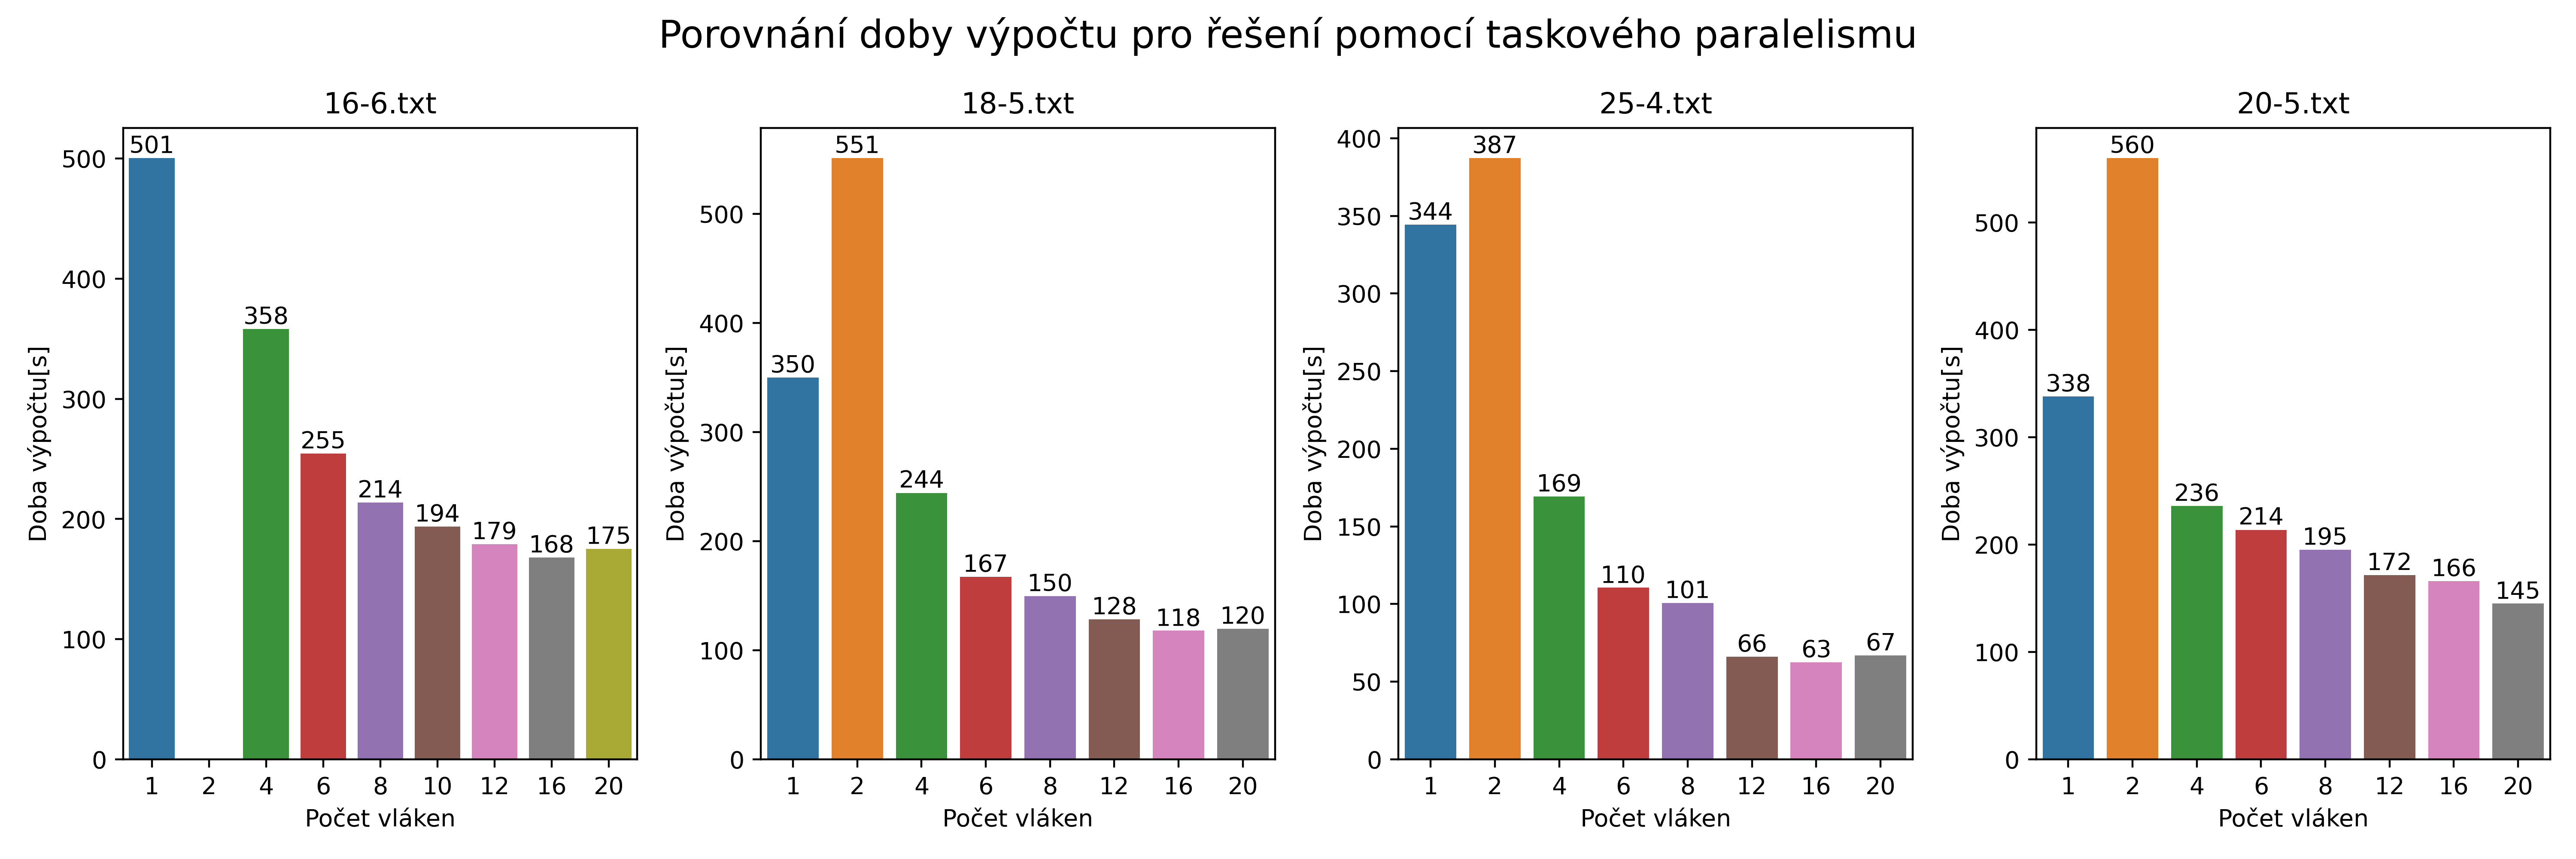
\includegraphics[scale=0.52]{report/images/parallel-task-graph.png}}
\caption{Porovnání doby výpočtu pro řešení pomocí taskového paralelismu}
\label{fig:task-graph.png}
\end{figure}
\FloatBarrier

Pro datový paralelismus byla zvolena hodnota \textbf{5} maximální hloubky, kde se nacházejí počáteční stavy.
Také byla vybrána na základě zkušeností získaných během semestru.
Je vidět stejná závislost jako v předchozím grafu, kdy s počtem vláken klesá doba výpočtu, úhel poklesu je však mnohem strmější.
Překvapivě je implementace algoritmu s jedním vláknem rychlejší než sekvenční, což je pravděpodobně způsobeno přípravou počátečních stavů.
Vyhledávací prostor je prohledán tak, že při rozdělení prostoru je větší šance, že se nejlepší stav nachází mezi prvními prohledávanými stavy, protože většina nejlepších stavů obsahuje téměř všechny hrany grafu.
Průběh poklesu je tentokrát na posledních 3 grafech výrazně odlišný.
Nejrychlejší doba běhu je asi \textbf{čtyřikrát} rychlejší než sekvenční implementace, a tedy \textbf{dvakrát} rychlejší než taskové paralelní řešení.
Po použití 20 vláken se přidání dalších nezdá být o tolik efektivnější.

\begin{figure}[!htbp]
\centerline{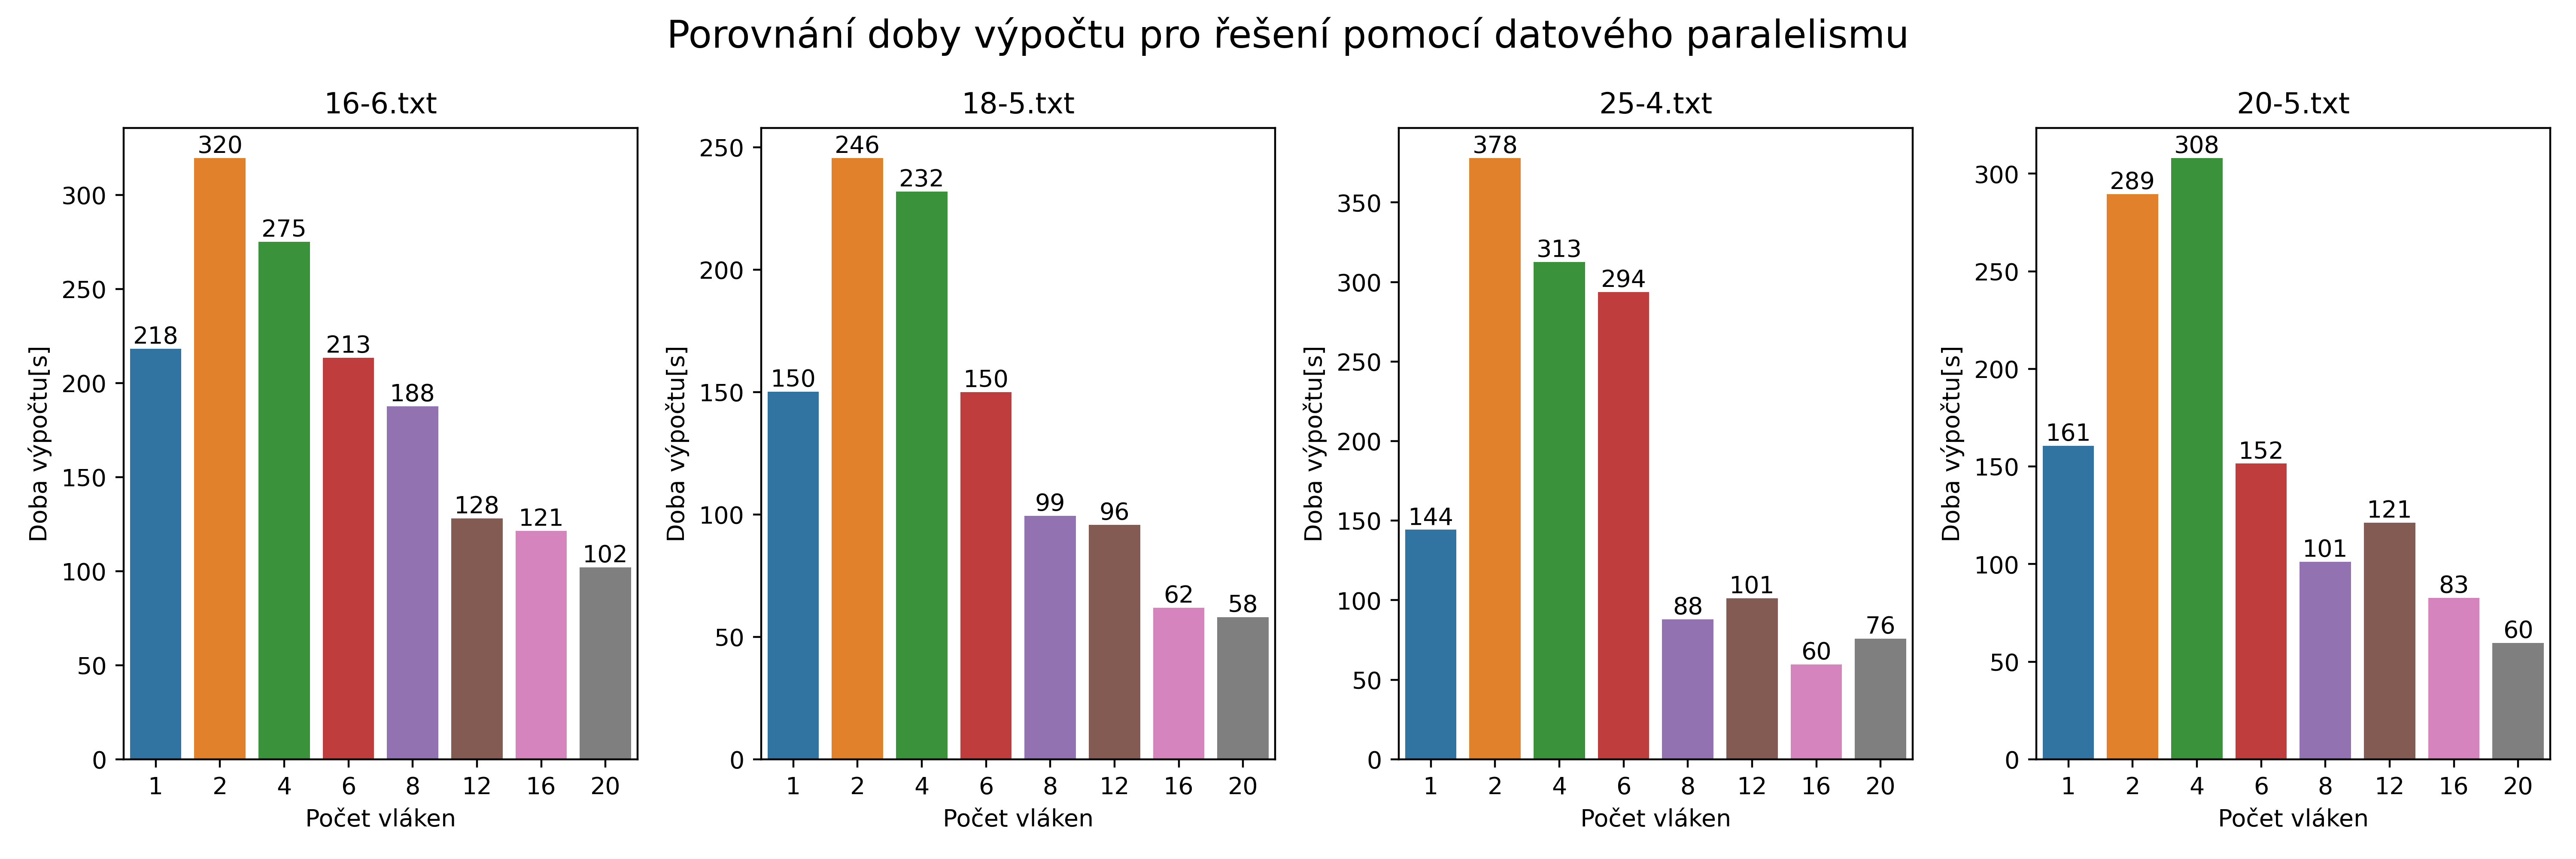
\includegraphics[scale=0.52]{report/images/parallel-data-graph.png}}
\caption{Porovnání doby výpočtu pro řešení pomocí datového paralelismu}
\label{fig:data-graph.png}
\end{figure}
\FloatBarrier

Nakonec byly porovnány výsledky distribuovaného řešení.
Maximální hloubka pro master proces byla zvolena \textbf{5} a pro slave procesy \textbf{6}.
Dokonce i většina běhů se 6 vlákny je rychlejší než nejrychlejší běh řešení pomocí datového paralelismu.
Doba výpočtu se neustále zkracuje a zhruba o polovinu se sníží od běhu se 6 vlákny k běhu s 20.
Ve srovnání s čistě paralelními řešeními se zdá, že má ještě větší potenciál běžet rychleji, pokud budou přidány nové výpočetní uzly nebo jádra.
Nejrychlejší běh každého grafu je asi \textbf{desetkrát} rychlejší než sekvenční, a proto asi \textbf{dvakrát až třikrát} rychlejší než implementace pomocí datového paralelismu.

\begin{figure}[!htbp]
\centerline{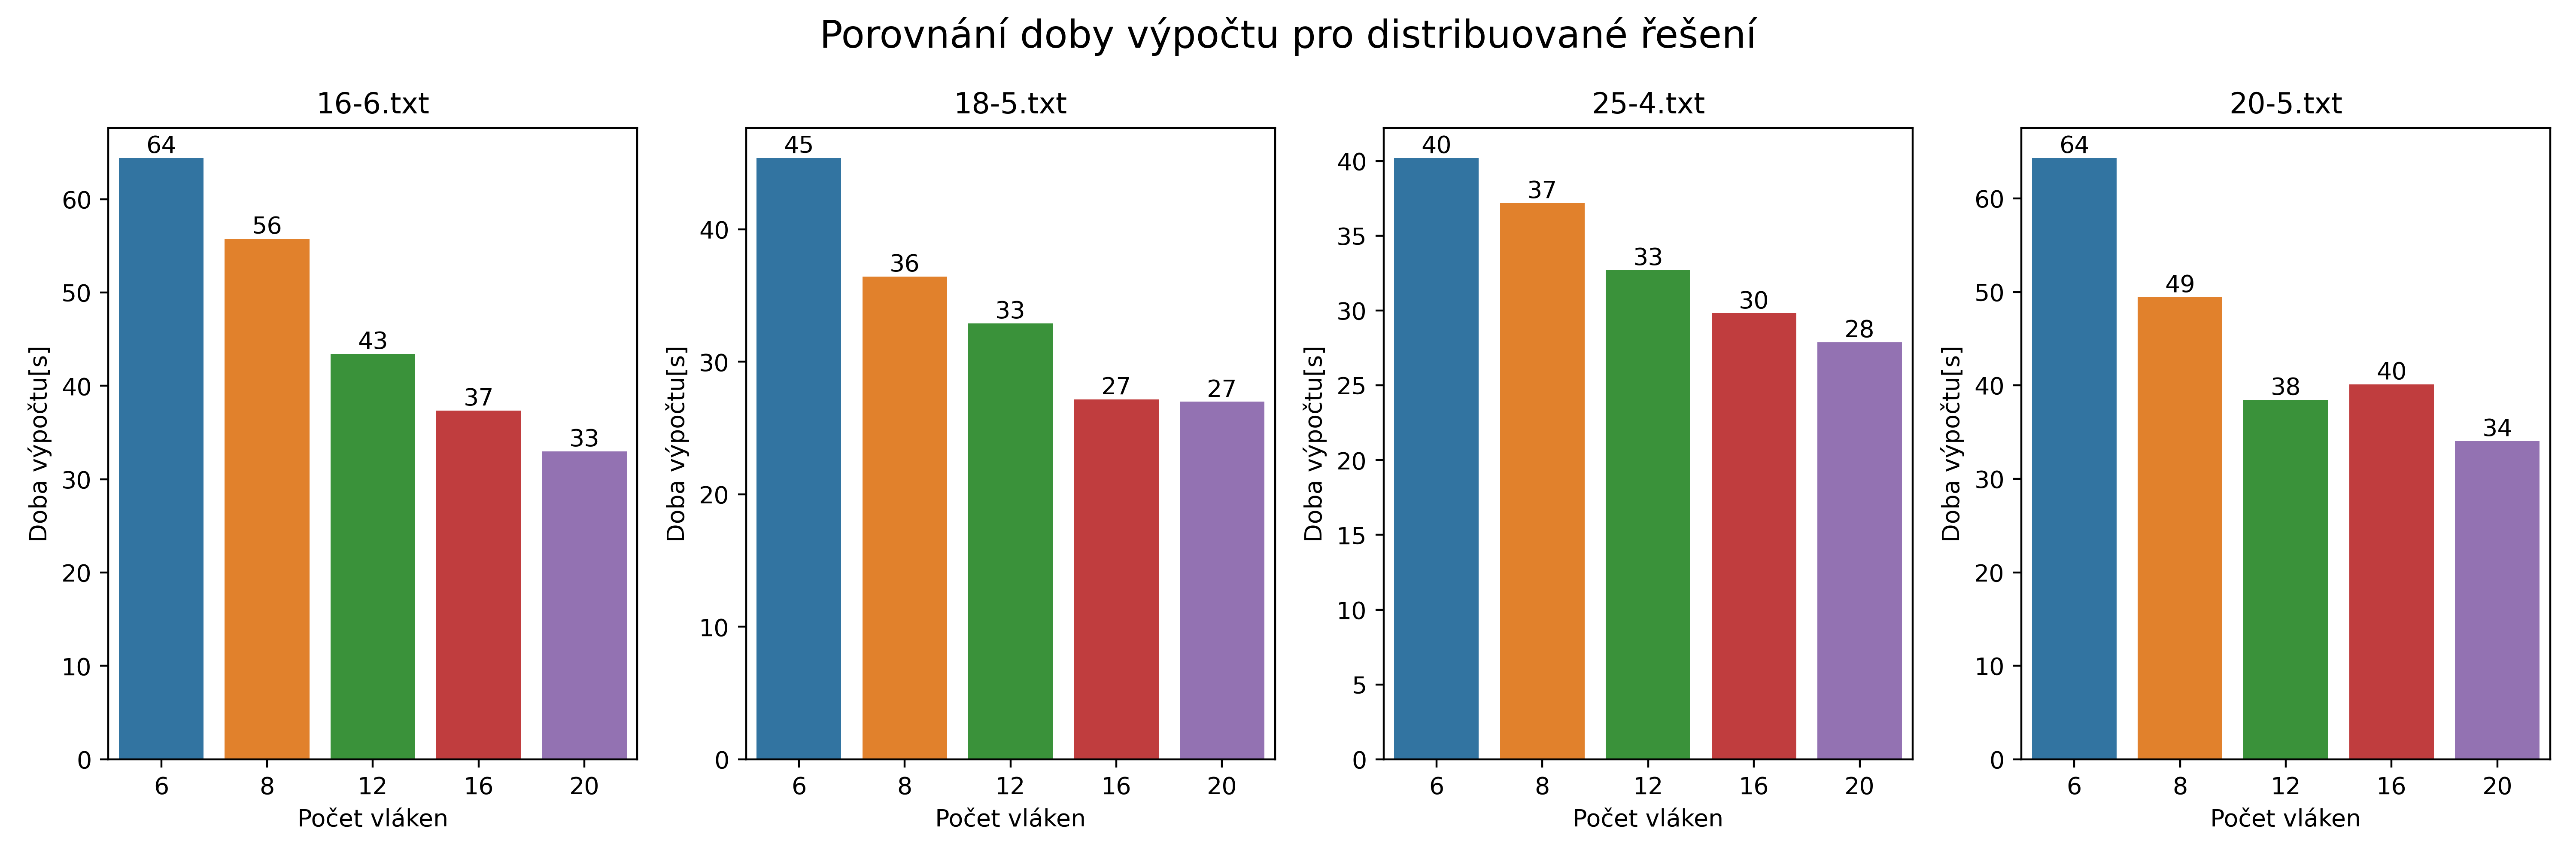
\includegraphics[scale=0.52]{report/images/distrib-graph.png}}
\caption{Porovnání doby výpočtu pro distribuované řešení}
\label{fig:distrib-graph.png}
\end{figure}
\FloatBarrier

Celkově se zdá, že implementace fungují dobře, protože algoritmus se s každou další implementací zrychloval.
V případě sekvenčního algoritmu by mohl běžet rychleji, pokud by se našel lepší způsob ořezávaní stavového prostoru, což by pravděpodobně urychlilo všechny následující implementace.
Realizace taskového paralelismu mohla být provedena jen o něco čitelněji.
V případě datového paralelismu je diskutabilní, zda použít samostatnou třídu pro sběr počátečních stavů, protože dělá kód složitější.
Místo DFS by stálo za zvážení použití prohledávání do šířky (BFS), jelikož dává algoritmu větší kontrolu nad počtem shromážděných stavů.

V případě distribuované implementace bylo vyvinuto úsilí o navázání komunikace mezi slave procesy, aby byl nejlepší stav aktuálnější.
Implementace však měla horší výsledky než jednodušší verze.
Ukázalo se, že je obtížné rozdělit paralelní část na dvě, z nichž jedna by sloužila pouze pro komunikaci a druhá pro výpočet.
OpenMP prostě nebylo takto navrženo.
Při zpětném pohledu na kód, nebylo třeba posílat graf a explorer pomocí instance \texttt{setting}, mohl to provést samotný podřízený proces.









